% -*- mode: latex; -*- mustache tags:  
\documentclass[10pt,twoside,english]{_support/latex/sbabook/sbabook}
\let\wholebook=\relax

\usepackage{import}
\subimport{_support/latex/}{common.tex}

%=================================================================
% Debug packages for page layout and overfull lines
% Remove the showtrims document option before printing
\ifshowtrims
  \usepackage{showframe}
  \usepackage[color=magenta,width=5mm]{_support/latex/overcolored}
\fi


% =================================================================
\title{Learning Object-Oriented Programming, Design and TDD with Pharo}
\author{Stéphane Ducasse}
\series{The Pharo TextBook Collection}

\hypersetup{
  pdftitle = {Learning Object-Oriented Programming, Design and TDD with Pharo},
  pdfauthor = {Stéphane Ducasse},
  pdfkeywords = {Introduction, programming, design, testing, Pharo, Smalltalk}
}


% =================================================================
\begin{document}

% Title page and colophon on verso
\maketitle
\pagestyle{titlingpage}
\thispagestyle{titlingpage} % \pagestyle does not work on the first one…

\cleartoverso
{\small

  Copyright 2017 by Stéphane Ducasse.

  The contents of this book are protected under the Creative Commons
  Attribution-ShareAlike 3.0 Unported license.

  You are \textbf{free}:
  \begin{itemize}
  \item to \textbf{Share}: to copy, distribute and transmit the work,
  \item to \textbf{Remix}: to adapt the work,
  \end{itemize}

  Under the following conditions:
  \begin{description}
  \item[Attribution.] You must attribute the work in the manner specified by the
    author or licensor (but not in any way that suggests that they endorse you
    or your use of the work).
  \item[Share Alike.] If you alter, transform, or build upon this work, you may
    distribute the resulting work only under the same, similar or a compatible
    license.
  \end{description}

  For any reuse or distribution, you must make clear to others the
  license terms of this work. The best way to do this is with a link to
  this web page: \\
  \url{http://creativecommons.org/licenses/by-sa/3.0/}

  Any of the above conditions can be waived if you get permission from
  the copyright holder. Nothing in this license impairs or restricts the
  author's moral rights.

  \begin{center}
    
\includegraphics[width=0.2\textwidth]{_support/latex/sbabook/CreativeCommons-BY-SA.pdf}
  \end{center}

  Your fair dealing and other rights are in no way affected by the
  above. This is a human-readable summary of the Legal Code (the full
  license): \\
  \url{http://creativecommons.org/licenses/by-sa/3.0/legalcode}

  \vfill

  % Publication info would go here (publisher, ISBN, cover design…)
  Layout and typography based on the \textcode{sbabook} \LaTeX{} class by Damien
  Pollet.
}


\frontmatter
\pagestyle{plain}

\tableofcontents*
\clearpage\listoffigures

\mainmatter

\chapter{Crafting a simple embedded DSL with Pharo}\label{cha:dsl}
In this chapter you will develop a simple domain specific language (DSL) for rolling dice. Players of games such as Dungeons \& Dragons are familiar with such DSL. An example of such DSL is the following expression: \textcode{2 D20 + 1 D6} which means that we should roll two 20-faces dices and one 6 faces die. 
It is called an embedded DSL because the DSL uses the syntax of the language used to implement it. Here we use the Pharo syntax to implement the Dungeons \& Dragons rolling die language. 

This little exercise shows how we can (1) simply reuse traditional operator such as \textcode{+}, (2) develop an embedded domain specific language and (3) use class extensions (the fact that we can define a method in another package than the one of the class of the method).
\section{Getting started}
Using the code browser, define a package named \textcode{Dice} or any name you like.
\subsection{Create a test }
It is always empowering to verify that the code we write is always working as we defining it. For this purpose you should create a unit test. Remember unit testing was promoted by K. Beck first in the ancestor of Pharo. Nowadays this is a common practice but this is always useful to remember our roots!

Define the class \textcode{DieTest} as a subclass of \textcode{TestCase} as follows: 

\begin{displaycode}{plain}
TestCase subclass: #DieTest
	instanceVariableNames: ''
	classVariableNames: ''
	package: 'Dice'
\end{displaycode}

What we can test is that the default number of faces of a die is 6. 

\begin{displaycode}{plain}
DieTest >> testInitializeIsOk
    self assert: Die new faces equals: 6
\end{displaycode}

If you execute the test, the system will prompt you to create a class \textcode{Die}. Do it.
\subsection{Define the class Die}
The class \textcode{Die} inherits from \textcode{Object} and it has an instance variable, \textcode{faces} to represent the number of faces one instance will have. Figure \ref{figOneClassDiceDesign} gives an overview of the messages. 


\begin{figure}

\begin{center}
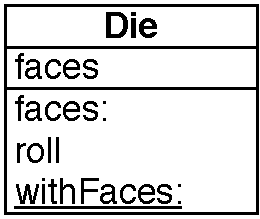
\includegraphics[width=0.25\textwidth]{/Users/ducasse/Workspace/FirstCircle/MyBooks/Bk-Writing/PharoBooks/LearningOOPWithPharoTrans/_result/pdf/Chapters/DSL/figures/OneClassDiceDesign.pdf}\caption{A single class with a couple of messages. Note that the method \textcode{withFaces:} is  a class method.\label{figOneClassDiceDesign}}\end{center}
\end{figure}


\begin{displaycode}{plain}
Object subclass:
	... Your solution ...
\end{displaycode}

In the \textcode{initialization} protocol, define the method \textcode{initialize} so that it simply sets the default number of faces to 6. 

\begin{displaycode}{plain}
Die >> initialize
	... Your solution ...
\end{displaycode}

Do not hesitate to add a class comment. 

Now define a method to return the number of faces an instance of \textcode{Die} has.

\begin{displaycode}{plain}
Die >> faces
	^ faces
\end{displaycode}

Now your tests should all pass (and turn green).
\section{Rolling a die}
To roll a die you should use the method from Number \textcode{atRandom} which draws randomly a 
number between one and the receiver. For example \textcode{10 atRandom} draws number between 1 to 10. 
Therefore we define the method \textcode{roll}:

\begin{displaycode}{plain}
Die >> roll
	... Your solution ...
\end{displaycode}

Now we can create an instance \textcode{Die new} and send it the message  \textcode{roll} and get a result.
Do \textcode{Die new inspect} to get an inspector and then type in the bottom pane \textcode{self roll}.
You should get an inspector like the one shown in Figure \ref{figDiceNoDetail}. With it you can interact with a die by writing expression in the bottom pane.


\begin{figure}

\begin{center}
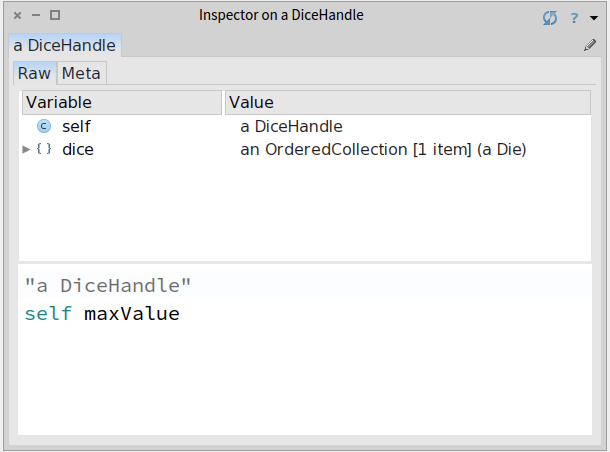
\includegraphics[width=0.6\textwidth]{/Users/ducasse/Workspace/FirstCircle/MyBooks/Bk-Writing/PharoBooks/LearningOOPWithPharoTrans/_result/pdf/Chapters/DSL/figures/DiceNoDetail.png}\caption{Inspecting and interacting with a die.\label{figDiceNoDetail}}\end{center}
\end{figure}


 
\section{Creating another test}
But better, let us define a test that verifies that rolling a new created dice with a default 6 faces only returns 
value comprised between 1 and 6. This is what the following test method is actually specifying.
 

\begin{displaycode}{plain}
DieTest >> testRolling
	| d |
	d := Die new.
	10 timesRepeat: [ self assert: (d roll between: 1 and: 6) ]
\end{displaycode}

\begin{important}
Often it is better to define the test even before the code it tests. Why? Because you can think about the API of your objects and a scenario that illustrate their correct behavior. It helps you to program your solution.
\end{important}
\section{Instance creation interface}
We would like to get a simpler way to create \textcode{Die} instances. For example we want to create a 20-faces die as follows: \textcode{Die withFaces: 20} instead of always have to send the new message to the class as in \textcode{Die new faces: 20}.
Both expressions are creating the same die but one is shorter.

Let us look at it: 

\begin{itemize}
\item In the expression \textcode{Die withFaces:}, the message \textcode{withFaces:} is sent to the class \textcode{Die}. It is not new, we constantly sent the message \textcode{new} to \textcode{Die} to created instances. 
\item Therefore we should define a method that will be executed 
\end{itemize}

Let us define a test for it.

\begin{displaycode}{plain}
DieTest >> testCreationIsOk
	self assert: (Die withFaces: 20) faces equals: 20
\end{displaycode}

What the test clearly shows is that we are sending a message to the \textbf{class} \textcode{Die} itself.
\subsection{Defining a class method}
Define the \textit{class} method \textcode{withFaces:} as follows:

\begin{itemize}
\item Click on the class button in the browser to make sure that you are editing a \textbf{class} method.
\item Define the method as follows: 
\end{itemize}

\begin{displaycode}{plain}
Die class >> withFaces: aNumber
	"Create and initialize a new die with aNumber faces."
	| instance |
	instance := self new.
	instance faces: aNumber.
	^ instance
\end{displaycode}

Let us explain this method

\begin{itemize}
\item The method \textcode{ withFaces:} creates an instance using the message \textcode{new}. Since \textcode{self} represents the receiver of the message and the receiver of the message is the class \textcode{Die} itself then \textcode{self} represents the class \textcode{Die}. 
\item Then the method sends the message \textcode{faces:} to the instance and 
\item Finally returns the newly created instance.
\end{itemize}

Pay really attention that a class method \textcode{withFaces:} is sent to a class, and an instance method sent to the newly created instance \textcode{faces:}. Note that the class method could have also named \textcode{faces:} or any name we want, it does not matter, it is executed when the receiver is the class \textcode{Die}.

This test will not work since we did not create yet the method \textcode{faces:}.  This is now the time to define it. Pay attention the method \textcode{faces:} is sent to an instance of the class \textcode{Die} and not the class itself. It is an instance method, therefore make sure that you deselected the class button before editing it.

\begin{displaycode}{plain}
Die >> faces: aNumber
	faces := aNumber
\end{displaycode}

Now your tests should run. So even if the class \textcode{Die} could implement more behavior, we are ready to implement a die handle. 

\begin{important}
A class method is a method executed in reaction to messages sent to a \textit{class}. It is defined on the class side of the class. In \textcode{Die withFaces: 20}, the message \textcode{withFaces:} is sent to the class \textcode{Die}. In \textcode{Die new faces: 20}, the message \textcode{new} is sent to the \textit{class} \textcode{Die} and the message \textcode{faces:} is sent to the \textit{instance} returned by \textcode{Die new}. 
\end{important}
\subsection{{[}Optional{]} Alternate instance creation definition}
 In a first reading you can skip this section. The \textit{class} method definition \textcode{withFaces:} above is strictly equivalent to the one below.

\begin{displaycode}{plain}
Die class >> withFaces: aNumber
	^ self new faces: aNumber; yourself
\end{displaycode}

Let us explain it a bit. \textcode{self} represents the class \textcode{Die} itself. Sending it the message \textcode{new}, we create an instance and send it the \textcode{faces:} message. And we return the expression. So why do we need the message \textcode{yourself}. The message \textcode{yourself} is needed to make sure that whatever value the instance message \textcode{faces:} returns, the instance creation method we are defining returns the new created instance. You can try to redefine the instance method \textcode{faces:} as follows:

\begin{displaycode}{plain}
Die >> faces: aNumber 
	faces := aNumber. 
	^ 33
\end{displaycode}

Without the use of \textcode{yourself}, \textcode{Die withFaces: 20} will return 33. With \textcode{yourself} it will return the instance.

The trick is that \textcode{yourself} is a simple method defined on \textcode{Object} class: The message \textcode{yourself} returns the receiver of a message.
The use of \textcode{;} sends the message to the receiver of the previous message (here \textcode{faces:}).  The message \textcode{yourself} is then sent to the object resulting from the execution of the expression \textcode{self new} (which returns a new instance of the class \textcode{Die}), as a consequence it returns the new instance. 
\section{First specification of a die handle}
Let us define a new class \textcode{DieHandle} that represents a die handle. 
The following code snippet shows the API that we would like to offer for now (as shown in Figure \ref{fig:DiceDesign}). We create a new handle then add some dice to it. We will use this kind of expressions in future tests below.


\begin{figure}

\begin{center}
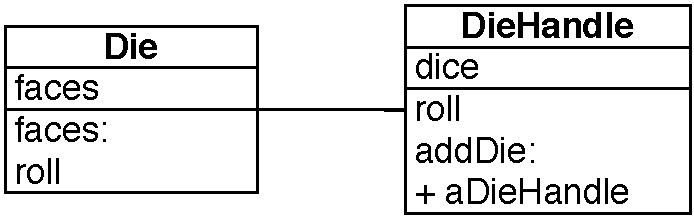
\includegraphics[width=0.6\textwidth]{/Users/ducasse/Workspace/FirstCircle/MyBooks/Bk-Writing/PharoBooks/LearningOOPWithPharoTrans/_result/pdf/Chapters/DSL/figures/DiceDesign.pdf}\caption{A die handle is composed of dice.\label{fig:DiceDesign}}\end{center}
\end{figure}


\begin{displaycode}{plain}
DieHandle new 
	addDie: (Die withFaces: 6);
	addDie: (Die withFaces: 10);
	yourself
\end{displaycode}

Of course we will define tests first for this new class. We define the class \textcode{DieHandleTest}.

\begin{displaycode}{plain}
TestCase subclass: #DieHandleTest
	instanceVariableNames: ''
	classVariableNames: ''
	package: 'Dice'
\end{displaycode}
\subsection{Testing a die handle}
We define a new test method as follows. We create a new handle and add one die of 6 faces and one die of 10 faces.
We verify that the handle is composed of two dice. 

\begin{displaycode}{plain}
DieHandleTest >> testCreationAdding
	| handle |
	handle := DieHandle new 
			addDie: (Die withFaces: 6);
			addDie: (Die withFaces: 10);
			yourself.
	self assert: handle diceNumber = 2.
\end{displaycode}

In fact we can do it better. Let us add a new test method to verify that we can even add
two dice having the same number of faces. 

\begin{displaycode}{plain}
DieHandleTest >> testAddingTwiceTheSameDice
	| handle |
	handle := DieHandle new. 
	handle addDie: (Die withFaces: 6).
	self assert: handle diceNumber = 1.
	handle addDie: (Die withFaces: 6).
	self assert: handle diceNumber = 2.
\end{displaycode}

Now that we specified what we want, we should implement the expected class and messages. 
Easy!
\section{Defining the DieHandle class}
The class \textcode{DieHandle} inherits from \textcode{Object} and it defines one instance variable to hold the dice it contains. 

\begin{displaycode}{plain}
Object subclass: ...
	... Your solution ...
\end{displaycode}

We simply initialize it so that its instance variable \textcode{dice} contains an instance of \textcode{OrderedCollection}.

\begin{displaycode}{plain}
DieHandle >> initialize
	... Your solution ...
\end{displaycode}

Then define a simple method \textcode{addDie:} to add a die to the list of dice of the handle. You can use the message \textcode{add:} sent to a collection.

\begin{displaycode}{plain}
DieHandle >> addDie: aDie 
	... Your solution ...
\end{displaycode}

Now you can execute the code snippet and inspect it. You should get an inspector as shown in Figure \ref{DieHandleNoDetail} 

\begin{displaycode}{plain}
DieHandle new 
	addDie: (Die withFaces: 6);
	addDie: (Die withFaces: 10);
	yourself
\end{displaycode}


\begin{figure}

\begin{center}
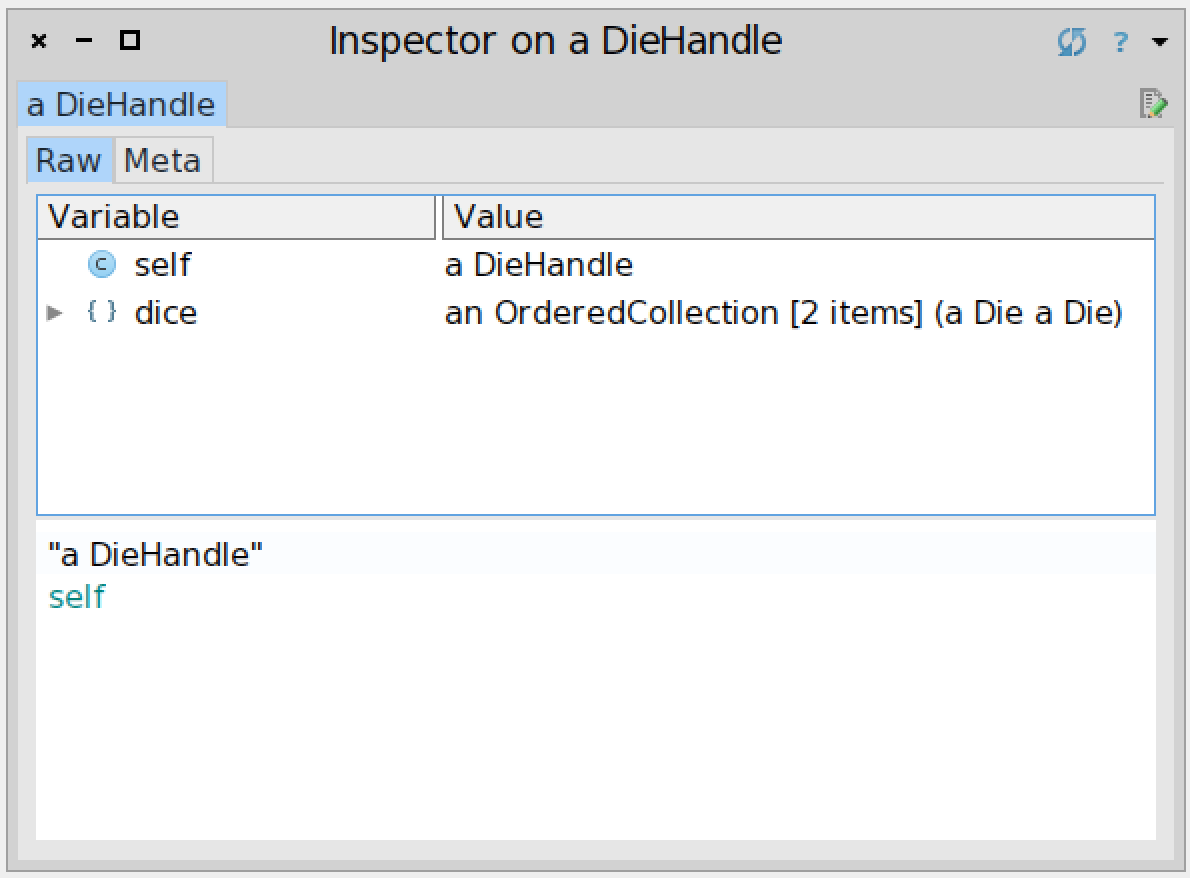
\includegraphics[width=0.6\textwidth]{/Users/ducasse/Workspace/FirstCircle/MyBooks/Bk-Writing/PharoBooks/LearningOOPWithPharoTrans/_result/pdf/Chapters/DSL/figures/DiceHandleNoDetail.png}\caption{Inspecting a DieHandle.\label{DieHandleNoDetail}}\end{center}
\end{figure}


Finally we should add the method \textcode{diceNumber} to the \textcode{DieHandle} class to be able to get the number of dice of the handle. We just return the size of the dice collection.

\begin{displaycode}{plain}
DieHandle >> diceNumber  
	^ dice size
\end{displaycode}

Now your tests should run and this is a good moment to save and publish your code. 
\section{Improving programmer experience}
Now when you open an inspector you cannot see well the dice that compose the die handle. Click on the \textcode{dice} instance variable and you will only get a list of \textcode{a Dice} without further information. What we would like to get is something like \textcode{a Die (6)} or \textcode{a Die (10)} so that in a glance we know the faces a die has. 

\begin{displaycode}{plain}
DieHandle new 
	addDie: (Die withFaces: 6);
	addDie: (Die withFaces: 10);
	yourself
\end{displaycode}

This is the  message \textcode{printOn:} that is responsible to provide a textual representation of the message receiver. By default, it just prints the name of the class prefixed with \textcode{'a'} or \textcode{'an'}. So we will enhance the \textcode{printOn:} method of the \textcode{Die} class to provide more information. Here we simply add the number of faces surrounded by parenthesis. The \textcode{printOn:} message is sent with a stream as argument. This is in such stream that we should add information. We use the message \textcode{nextPutAll:} to add a number of characters to the stream. We concatenate the characters to compose \textcode{()} using the message \textcode{,} comma defined on collections (and that concatenate collections and strings).

\begin{displaycode}{plain}
Die >> printOn: aStream

	super printOn: aStream.
	aStream nextPutAll: ' (', faces printString, ')'
\end{displaycode}

Now in your inspector you can see effectively the number of faces a die handle has as shown by Figure \ref{diceDetail} and it is now easier to check the dice contained inside a handle (See Figure \ref{DieHandleDetail}).


\begin{figure}

\begin{center}
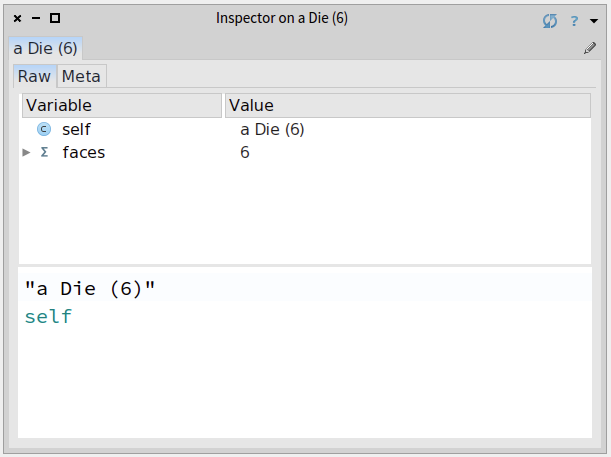
\includegraphics[width=0.7\textwidth]{/Users/ducasse/Workspace/FirstCircle/MyBooks/Bk-Writing/PharoBooks/LearningOOPWithPharoTrans/_result/pdf/Chapters/DSL/figures/DiceDetail.png}\caption{Die details.\label{diceDetail}}\end{center}
\end{figure}
 


\begin{figure}

\begin{center}
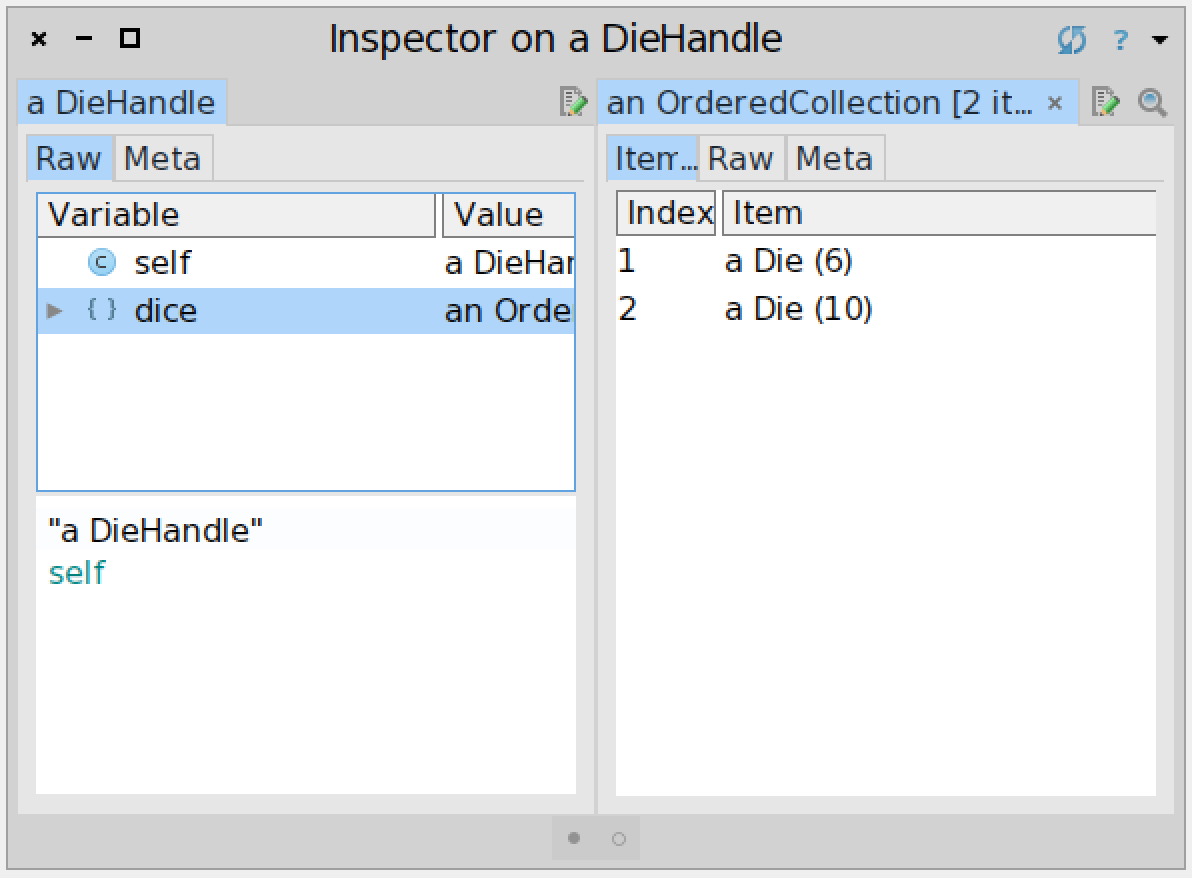
\includegraphics[width=0.9\textwidth]{/Users/ducasse/Workspace/FirstCircle/MyBooks/Bk-Writing/PharoBooks/LearningOOPWithPharoTrans/_result/pdf/Chapters/DSL/figures/DiceHandleDetail.png}\caption{A die handle with more information.\label{DieHandleDetail}}\end{center}
\end{figure}
 

\textbf{Note} This implementation of \textcode{printOn:} is suboptimal. Indeed during the message \textcode{faces printString}, it creates a separate stream instead of using the one pass as argument.
To understand the problem you can have a look at the implementation of the method \textcode{printString} defined in the class \textcode{Object}. 

\begin{displaycode}{plain}
Die >> printOn: aStream
	
	super printOn: aStream.
	aStream 
		nextPutAll: '(';
		print: faces; 
		nextPutAll: ')'
\end{displaycode}
\section{Rolling a die handle}
Now we can define the rolling of a die handle by simply summing result of rolling each of its dice. 
Implement the \textcode{roll} method of the \textcode{DieHandle} class. This method must collect the results of rolling each dice of the handle and sum them.

You may want to have a look at the method \textcode{sum:} in the class \textcode{Collection} or use a simple loop such as \textcode{do:} to iterate over the dice.

\begin{displaycode}{plain}
DieHandle >> roll
	... Your solution ...
\end{displaycode}

Now we can send the message \textcode{roll} to a die handle.

\begin{displaycode}{plain}
handle := DieHandle new 
		addDie: (Die withFaces: 6);
		addDie: (Die withFaces: 10);
		yourself.
handle roll
\end{displaycode}

Define a test to cover such behavior. Rolling an handle of n dice should be between n and the sum of the face number of each die. 

\begin{displaycode}{plain}
DieHandleTest >> testRoll
	... Your solution ...
\end{displaycode}
\section{About Dice and DieHandle API}
It is worth to spend some times looking at the relationship between \textcode{DieHandle} and \textcode{Dice}. 
A die handle is composed of dices. What is an important design decision is that the API of the main behavior (\textcode{roll}) is the same for a die or a die handle. You can send the message \textcode{roll} to a dice or a die handle. This is an important property.

Why? Because it means that from a client perspective, she/he can treat the receiver without having to take care about the kind of object it is manipulating. A client just sends the message \textcode{roll} to an object and get back a number (as shown in Figure \ref{figDieHandleComposition}). The client is not concerned by the fact that the receiver is composed out a simple object or a complex one. Such design decision supports the \textit{Don't ask, tell} principle.


\begin{figure}

\begin{center}
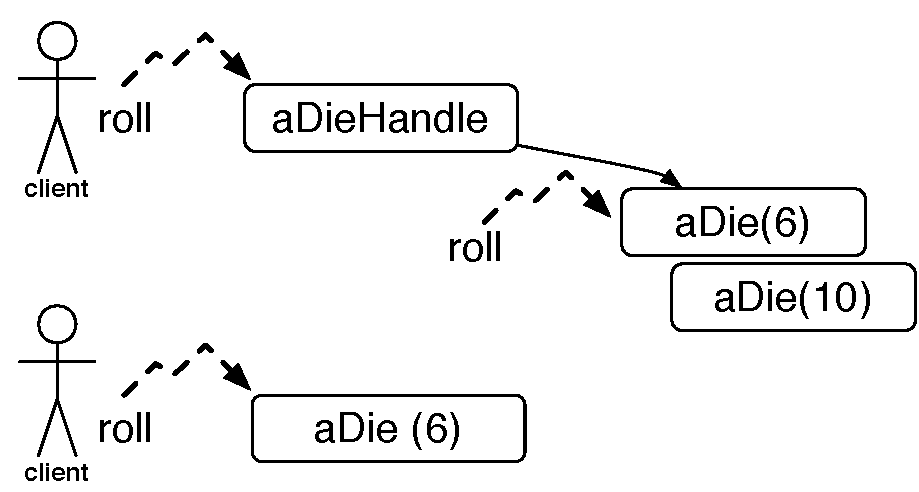
\includegraphics[width=0.6\textwidth]{/Users/ducasse/Workspace/FirstCircle/MyBooks/Bk-Writing/PharoBooks/LearningOOPWithPharoTrans/_result/pdf/Chapters/DSL/figures/DiceHandleComposition.pdf}\caption{A polymorphic API supports the \textit{Don't ask, tell} principle.\label{figDieHandleComposition}}\end{center}
\end{figure}


\begin{important}
Offering polymorphic API is a tenet of good object-oriented design. It enforces the \textit{Don't ask, tell} principle. Clients do not have to worry about the type of the objects to whom they talk to. 
\end{important}

For example we can write the following expression that adds a die and a dieHandle to a collection and collect the different values (we convert the result into an array so that we can print it in the book).

\begin{displaycode}{plain}
| col |
col := OrderedCollection new. 
col add: (Die withFaces: 20).
col add: (DieHandle new addDie: (Die withFaces: 4); yourself).
(col collect: [:each | each roll]) asArray
>>> #(17 3) 
\end{displaycode}
\subsection{About composition}
Composite objects such document objects (a book is composed of chapters, a chapter is composed of sections, a section is composed of paragraphs) have often a more complex composition relationship than the composition between die and die handle. Often the composition is recursive in the sense that an element can be the whole: for example, a diagram can be composed of lines, circles, and other diagrams. We will see an example of such composition in the Expression Chapter \ref{cha:expressions}.
\section{Role playing syntax}
Now we are ready to offer a syntax following practice of role playing game, i.e., using \textcode{2 D20} to create a handle of two dice with 20 faces each.  For this purpose we will define class extensions: we will define methods in the class \textcode{Integer} but these methods will be only available when the package Dice will be loaded. 

But first let us specify  what we would like to obtain by writing a new  test in the class \textcode{DieHandleTest}. Remember
to always take  any opportunity to write tests.  When we execute \textcode{2 D20} we  should get a new handle  composed of two
dice and can verify that. This is what the method \textcode{testSimpleHandle} is doing.

\begin{displaycode}{plain}
DieHandleTest >> testSimpleHandle
	self assert: 2 D20 diceNumber = 2.
\end{displaycode}

Verify that the test is not working! It is much more satisfactory to get a test running when it was not working before. Now define the method \textcode{D20} with a protocol named \textcode{*NameOfYourPackage} (\textcode{'*Dice}' if you named your package \textcode{'Dice'}).
The \textcode{*} (star) prefixing a protocol name indicates that the protocol and its methods belong to another package than the package of the class. Here we want to say that while the method \textcode{D20} is defined in the class \textcode{Integer}, it should be saved with the package \textcode{Dice}. 
 
The method \textcode{D20} simply creates a new die handle, adds the correct number of dice to this handle, and returns the handle.

\begin{displaycode}{plain}
Integer >> D20
	... Your solution ...
\end{displaycode}
\subsection{About class extensions}
We asked you to place the method \textcode{D20} in a protocol starting with a star and having the name of the package (\textcode{'*Dice'}) because we want this method to be saved (and packaged) together with the code of the classes we already created (\textcode{Die}, \textcode{DieHandle},...) 
Indeed in Pharo we can define methods in classes that are not defined in our package. Pharoers call this action a class extension: we can add methods to a class that is not ours. For example \textcode{D20} is defined on the class \textcode{Integer}. Now such methods only make sense when the package \textcode{Dice} is loaded. 
This is why we want to save and load such methods with the package we created. This is why we are defining the protocol as \textcode{'*Dice'}.
This notation is a way for the system to know that it should save the methods with the package and not with the package of the class \textcode{Integer}. 

Now your tests should pass and this is probably a good moment to save your work either by publishing your package and to save your image. 

We can do the same for the default dice with different faces number: 4, 6, 10, and 20. But we should avoid duplicating logic and code. So first we will introduce a new method \textcode{D:} and based on it we will define all the others.

Make sure that all the new methods are placed in the protocol \textcode{'*Dice'}. To verify you can press the button Browse of the Monticello package browser and you should see the methods defined in the class \textcode{Integer}. 

\begin{displaycode}{plain}
Integer >> D: anInteger
	... Your solution ...
\end{displaycode}

\begin{displaycode}{plain}
Integer >> D4
	^ self D: 4
\end{displaycode}

\begin{displaycode}{plain}
Integer >> D6
	^ self D: 6
\end{displaycode}

\begin{displaycode}{plain}
Integer >> D10
	^ self D: 10
\end{displaycode}

\begin{displaycode}{plain}
Integer >> D20
	^ self D: 20
\end{displaycode}

We have now a compact form to create dice and we are ready for the last part: the addition of handles. 
\section{Handle's addition}
Now what is missing is that possibility to add several handles as follows: \textcode{2 D20 + 3 D10}. Of course let's write a test first to be clear on what we mean.

\begin{displaycode}{plain}
DieHandleTest >> testSumming
	| handle |
	handle := 2 D20 + 3 D10.
	self assert: handle diceNumber = 5.
\end{displaycode}

We will define a method \textcode{+} on the \textcode{DieHandle} class. In other languages this is often not possible or is based on operator overloading. In Pharo \textcode{+} is just a message as any other, therefore we can define it on the classes we want.

Now we should ask ourself what is the semantics of adding two handles. Should we modify the receiver of the expression or create a new one. We preferred a more functional style and choose to create a third one. 

The method \textcode{+} creates a new handle then add to it the dice of the receiver and the one of the handle passed as argument to the message. Finally we return it. 

\begin{displaycode}{plain}
DieHandle >> + aDieHandle
	... Your solution ... 
\end{displaycode}

Now we can execute the method \textcode{(2 D20 + 1 D6) roll} nicely and start playing role playing games, of course.
\section{Conclusion}
This chapter illustrates how to create a small DSL based on the definition of some domain classes (here \textcode{Dice} and  
 \textcode{DieHandle}) and the extension of core class such as \textcode{Integer}. It also shows that we can create packages with all the methods that are needed even when such methods are defined on classes external (here \textcode{Integer}) to the package.  
It shows that in Pharo we can use usual operators such as \textcode{+} to express natural models.


% lulu requires an empty page at the end. That's why I'm using
% \backmatter here.
\backmatter

% Index would go here
\bibliographystyle{abbrv}
\bibliography{others.bib}
\end{document}
